\documentclass[../Report.tex]{subfiles}

\begin{document}

This project is composed of a set of Python scripts that run the benchmark, analyse the results and create the confusion matrix along with some statistics. 
The generation of the final results can be accomplished in 2 steps running the following scripts:

\begin{enumerate}
	\item \texttt{run\_test.py} Runs the Maven compilation of the benchmark together with the
	Infer quandary tool and exports the results. Note that Infer is launched with the option
	--quandary-only, thus the results are all and only those obtained by the Quandary plugin. 
	\item \texttt{confusion\_builder.py} For each exported result from the previous step, prints statistics and the confusion matrix.
\end{enumerate}

\subsection{Custom Infer configurations}
As mentioned before, it is possible to customise the analysis of vulnerabilities performed by Quandary providing an ad-hoc configuration file. Here it is possible to setup some custom sinks, endpoints, sources and sanitizers. In the project, we provide this configuration in the file \emph{.inferconfig}. We focus here on the definition of sanitizing procedure, as the one for sources and sinks is quite straightforward. \\
We declare as sanitizers the following procedures:
\begin{itemize}
	\item \emph{decodeForHTML}, \emph{decodeFromBase64}, \emph{decodeFromURL},
	\emph{canonicalize} and \emph{encodeForHTML} defined in org.owasp are
	pretty standard, and can be used to remove dangerous characters from the 
	input;
	\item as unsecure random number generation is a flaw, the java standard Random is not
	considered to be a sanitizer. Instead, we allow as a sanitizer the \emph{SecureRandom}
	procedure defined in the java.security framework;
	\item encryption using SHA is always considered to be a sanitizer. Note that, as we have
	no way to specify which SHA algorithm are going to use, Quandary is not able to report
	a vulnerabilty caused by the usage of an unsecure algortihm, as for instance SHA1: more
	on this later on. A similar consideration can be done for the last sanitizer, the 
	\emph{MessageDigest} procedure defined in java.security.
\end{itemize}
In order to run the test with a different configuration it is only needed to edit this configuration file and run again the tool as descrived above.

\subsection{Compare the results}
Each time the \texttt{run\_test.py} script is run, a \texttt{csv/actual/actual.csv} file is generated or overwritten. The csv file mirrors the one provided in the owasp benchmark, hence having the fields:
\begin{itemize}
	\item \emph{filename} the name of the java test file;
	\item \emph{vulnerability name} the name of the vulnerability considered by the test;
	\item \emph{vulnerability presence} a boolean flag indicating wheter the vulnerability is
	present or not;
	\item \emph{CWE number} the number associated to the vulnerabilty in the Common Weakness
	Enumeration.
\end{itemize}
The structure of the file is shown in fig.~\ref{img:csv}.

\begin{figure}
	\begin{center}
		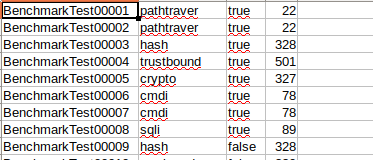
\includegraphics[scale=0.5]{res.png}
	\end{center}
	\caption{The expected results csv}
	\label{img:csv}
\end{figure}

Note that, as the vulnerability name and CWE number are not useful for the analysis, we basically ignore them when building the results csv.
In order to compare different results from different configurations of the Quandary tool and assess the results, it is possible to rename this file and run again the script: the new configuration is automatically recognized by Quandary. In this case, a new \texttt{csv/actual/actual.csv} file will be generated and the old one won't be overwritten. As the confusion matrix builder can build up the matrix for different csv files, running again the script will results in getting separate statistics according to all the \texttt{.csv} files placed inside the \texttt{csv/actual} folder, hence easing the comparison between different configurations.

\end{document}